\chapter{Experiment} \label{ch:experiment}

\section{Radioactive Ion Beam Factory(RIBF) at RIKEN}

\begin{figure}[h!]
\centering
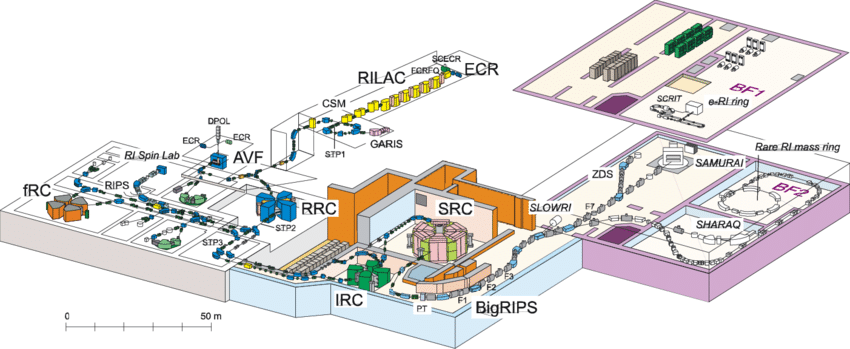
\includegraphics[width=15cm, height=11cm]{figures/Layout-of-the-RIKEN-RI-Beam-Factory.png}
\caption[Layout of the RIBF showing various accelerators]{Layout of the RIBF showing various accelerators and the BigRIPS ion separator \citep{rikenasc}. }
\end{figure}
The RIBF is world-class fragmentation ion beam facility. It is part of physics division at RIKEN, Japan. The facility consists of a 22 year old facility(since 1986) and a new facility which has been completed recently. The old facility has the heavy-ion accelerator complex consisting of a K540-MeV ring cyclotron (RRC) and its two injectors: a variable-frequency heavy-ion linac (RILAC) and a K70-MeV AVF cyclotron (AVF). These accelerators have been providing a lot of users in various research fields with the world’s most intense ion beams over the whole range of elements. The RILAC provides a heavy-ion beam with energy up to 6 MeV/nucleon. The AVF provides protons up to 14 MeV and Ca ions up to 5.6MeV/nucleon. The RRC can provide protons up to 210 MeV, heavy ions such as C, O and Ne ions up to 135MeV/nucleon, Ar ions up to 95 MeV/nucleon and Bi ions up to 15 MeV/nucleon. Moreover, the projectile-fragment separator at the RRC (RIPS) provides the world's most intense low-atomic-mass (\textless 60) RI beams.

The RIBF has very recently added new dimensions to the facility's capabilities: a new high-power heavy-ion booster system consisting of three ring cyclotrons with K=570 MeV (fixed frequency, fRC), 980 MeV (intermediate stage, IRC) and 2500 MeV (superconducting, SRC), respectively, can boost energies of the output beams from the RRC up to 440 MeV/nucleon for light ions and 350 MeV/nucleon for very heavy ions. The goal of the available intensity is set to be 1 p$\mu$A, which is limited due to presently planned radiation shielding power around a primary-beam dump. The superconducting isotope separator, BigRIPS, converts these energetic heavy-ion beams into intense RI beams via the projectile fragmentation of stable ions or the in-flight fission of uranium ions. The combination of the SRC and the BigRIPS expands our nuclear world on the nuclear chart into \textit{terra incognita}. 

\begin{figure}[h!]
\centering
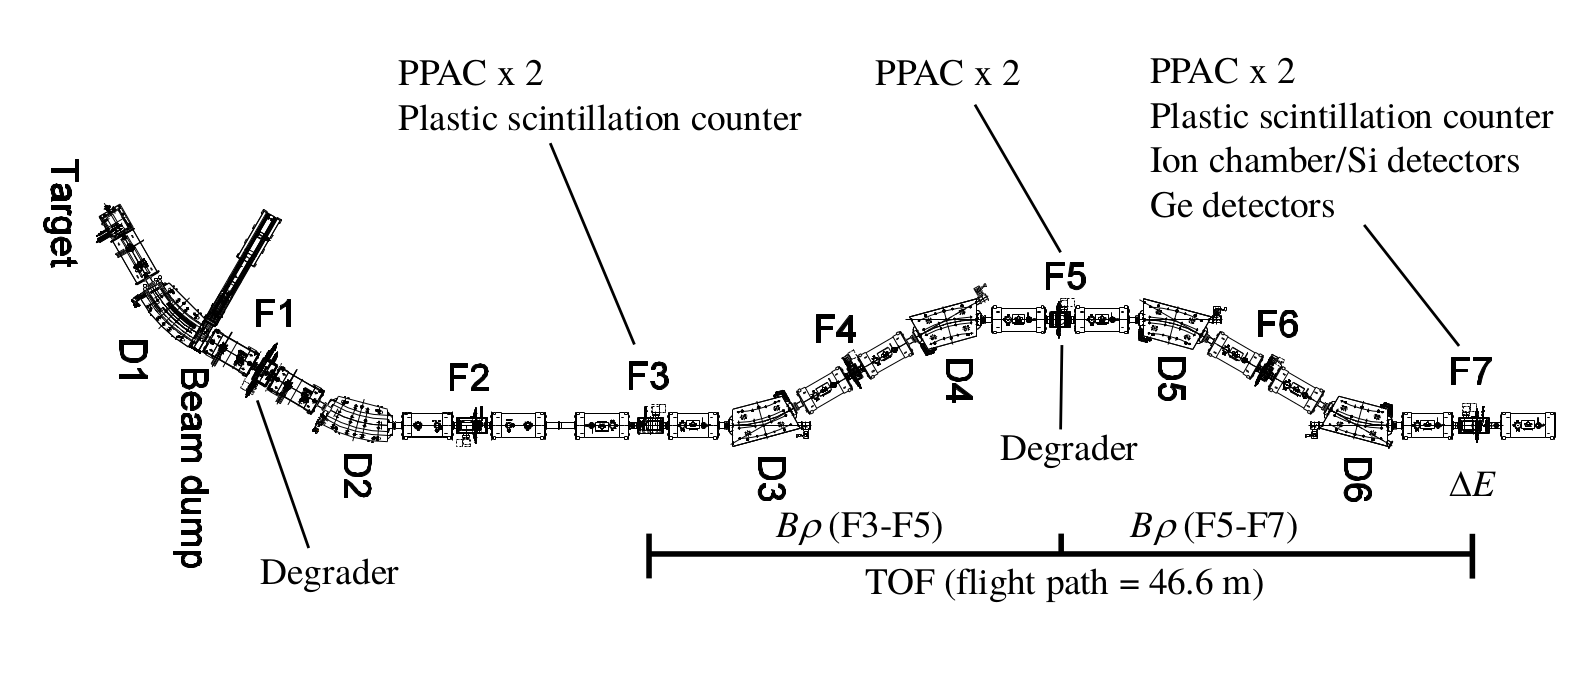
\includegraphics[width=19cm, height=11cm, angle=90]{figures/bigrips.png}
\caption[Schematic diagram of the BigRIPS separator]{Schematic diagram of the BigRIPS separator at RIBF. The first stage includes the components from the production target (F0) to F2, while the second stage spans those from F3 to F7 \citep{FUKUDA2013323}.}
\end{figure}

BigRIPS is an in-flight RI beam separator available at RIBF for the production of intense RI beams with a wide range of masses and isospin. The characteristic features of the BigRIPS separator are large ion-optical acceptances and a two-stage structure. The angular acceptances are $\pm$40 mrad horizontally and $\pm$50 mrad vertically, and the momentum acceptance is
$\pm$3 $\%$, allowing efficient collection of fragments produced by not only projectile fragmentation but also in-flight fission of a
\textsuperscript{238}U beam. The large acceptances are achieved by the use of superconducting quadrupoles with large apertures. The two-stage structure allows delivery of tagged RI beams and two-stage isotope separation. The first stage of the BigRIPS separator is used for production, collection, and separation of RI beams with an energy degrader, while particle identification of RI beams (separator-spectrometer mode) and/or further isotope separation with another energy degrader (separator-separator mode) are performed in the second stage. The particle identification is based on the TOF-B$\rho$ -$\Delta$E method, in which the time of flight (TOF), magnetic rigidity (B$\rho$ ), and energy loss ($\Delta$E) are measured to deduce the atomic number (Z) and the mass-to-charge ratio (A/Q) of RI beams. Such in-flight particle identification is an essential requirement for delivering tagged RI beams, making it possible to perform various types of experiments including secondary reaction measurements. Since the total kinetic energy is not measured in this scheme, and consequently A and Q cannot be determined independently, the resolution in A/Q must be high enough to identify the charge state Q of RI beams. Furthermore, the flight path is fairly long (46.6 m), so that the TOF value can be determined with fairly high resolution.



\subsection{YSO implementation in BRIKEN experiment}

The YSO detector was used for the first time at RIBF, RIKEN for two consecutive experiments. It was implemented as a part of the BRIKEN \citep{BRIKEN} neutron counter already present at the facility. The YSO detector was used as one of the implant detectors along with WAS3ABI and AIDA. The PSPMT of the detector was optimized to operate at a biasing voltage of 575 V to get the desired dynamic range for the ions, and the betas. The experiments involved accelerating \textsuperscript{238}U upto 345 MeV/nucleon with a charge state of (86+) which is the primary beam, followed by hitting a 4 mm thick rotating target of \textsuperscript{9}Be.
\begin{figure}[h]
    \centering
    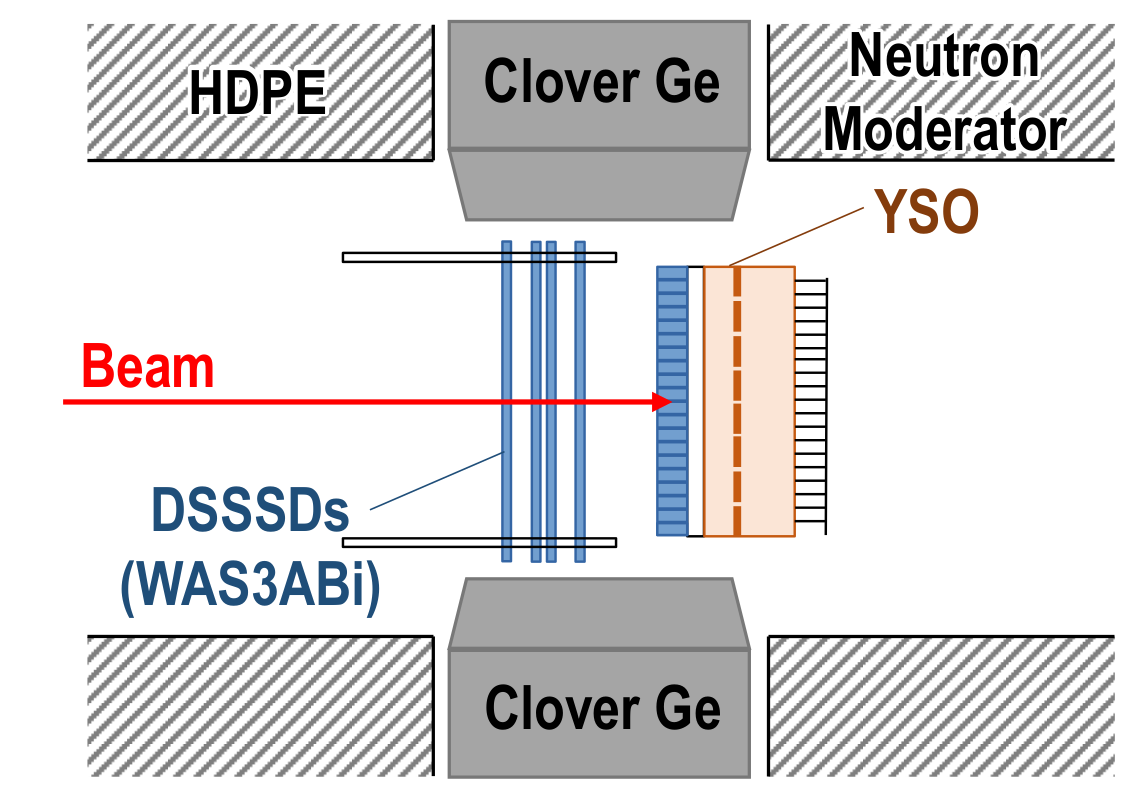
\includegraphics[width=10cm,height=8cm]{figures/experimental_setup.png}
    \caption[A diagram showing the instrumental setup for the]{A diagram showing the instrumental setup for the experiment as viewed from above. WAS3ABi and YSO are placed in a cavity at the center of BRIKEN neutron detector, approximately 2 cm apart. This position geometrically ensures detection of maximum possible neutrons (prompt and delayed) by the neutron counter. The High Density Polyethylene (HDPE) is used to moderate energetic delayed neutrons, advancing them in a region of high interaction cross-section with the \textsuperscript{3}He tubes comprising the BRIKEN neutron counter. Two High purity germanium clover detectors were employed to record the $\beta$-correlated $\gamma$-rays.}
    \label{fig:experimental}
\end{figure} 
The reaction leads to the synthesis of a gamut of exotic isotopes which are tagged and separated by BigRIPS facility on an event by event basis. This tagged  secondary beam of ions provided by the BigRIPS facility was implanted onto the detector with a particular combination of aluminum degraders, required to monitor the energy and range of ions. The first experiment had a secondary beam centered around \textsuperscript{82}Cu, and the second experiment itself involved
two mass settings. The first setting involved nuclei around \textsuperscript{115}Nb and the second setting provided nuclei centered around \textsuperscript{100}Br. 
The five signals (four positions and one energy) from the detector were split and used with different gain settings. One set of signals was devoted to implant position and energy measurements with no amplification. The other set was used for calculating the energy and position of the betas, with an amplification $\sim$ 10 for obtaining a good signal-to-noise ratio leading to better estimates of energy as well as position in the \textit{x-y} plane of the detector.


\begin{figure}[h!]
    \centering
    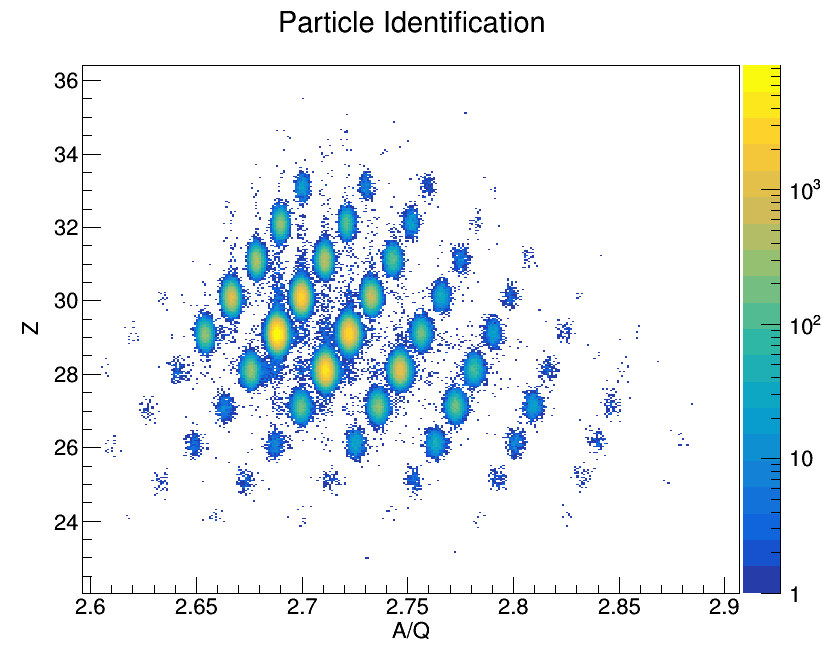
\includegraphics[width=10cm, height=8cm]{figures/yso_pid_2.png}
    \caption[Particle identification plot for ions stopped in YSO]{Particle identification plot for ions stopped in YSO. This information is provided by the BigRIPS facility and is important for ion-specific analysis.}
    \label{fig:particleidentification}
\end{figure}

\subsubsection{Ion-$\beta$ Correlations}
The essential purpose of the implantation detector is to establish the correlations between implanted ions and the corresponding $\beta$-decay electrons. These correlations are implemented by using a position-gate around the position of the implanted ion in the \textit{x-y} plane. The gate is optimized to achieve a high beta efficiency, thus maximum signal-to-noise ratio. 

The correlations are used in calculating half-lives of various isotopes and to further investigate the decay chains involving neutrons. The correlations were verified by calculating the half-lives of the known isotopes. Figure \ref{fig:ysocorrelations} shows the correlations between $\beta$ and implantation events. The correlation is manifested in the form of a hot-spot in the implant image in the vicinity of the $\beta$-event on the image scale. 

\begin{figure}[h!]
    \centering
    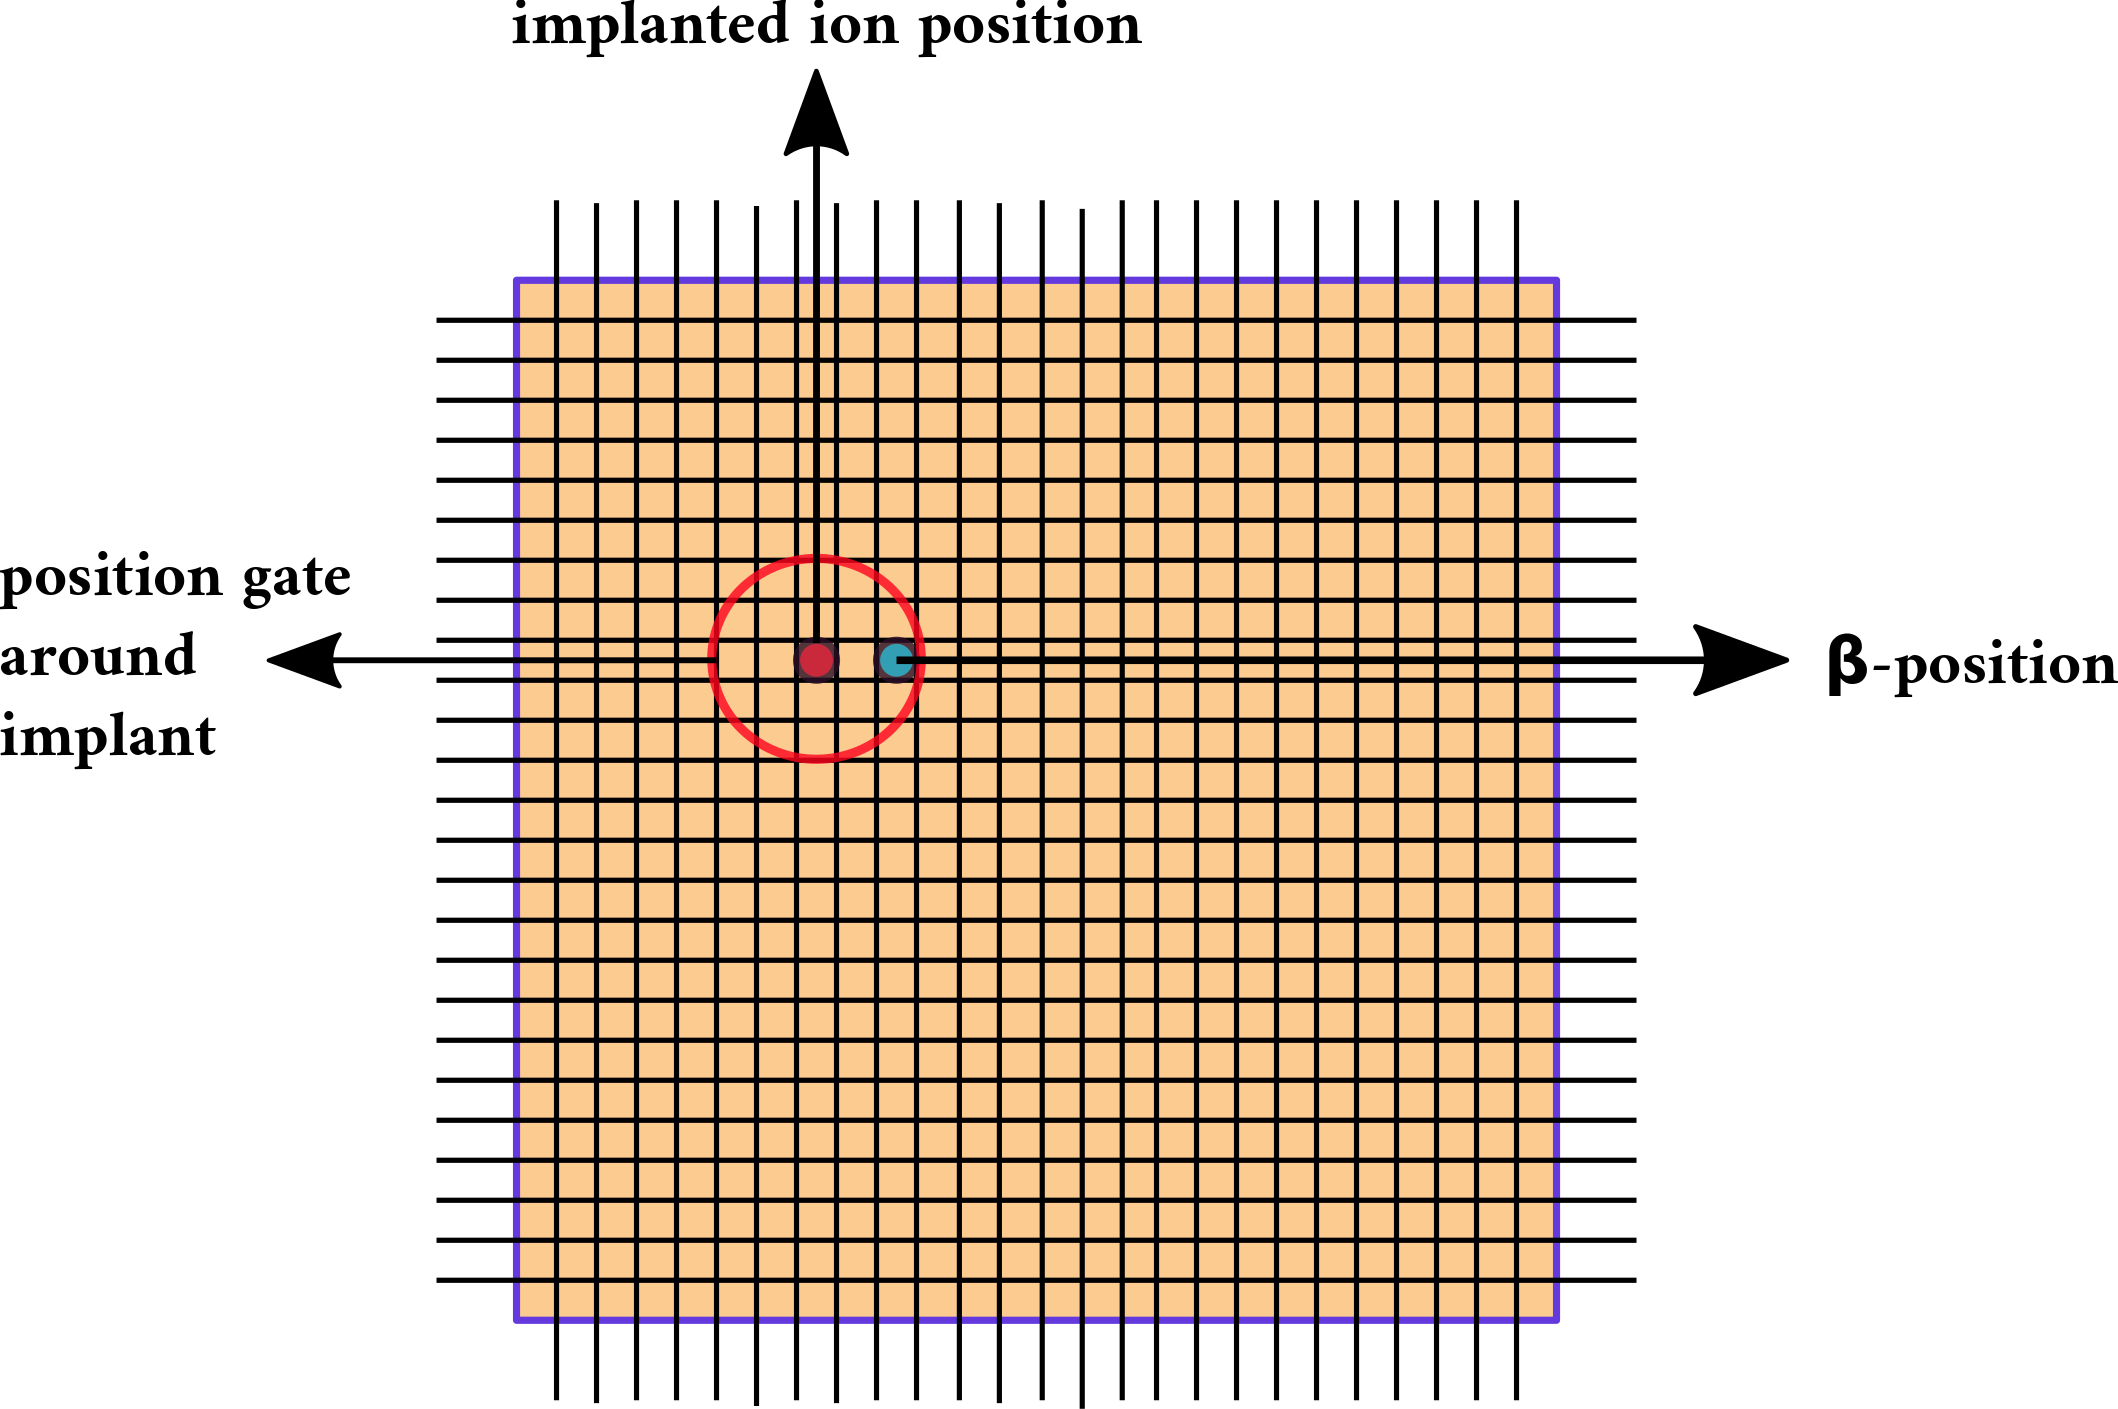
\includegraphics[width=12cm,height=8cm]{figures/pastedImage.png}
    \caption[A graphical representation of the algorithm devised to identify ion-beta]{A graphical representation of the algorithm devised to identify ion-beta correlations, showing a valid association. The diagram shows ion and beta position with red and blue shaded circles, respectively.}
    \label{fig:ion_beta_correlations}
\end{figure}

\begin{figure}[h!]
    \centering
    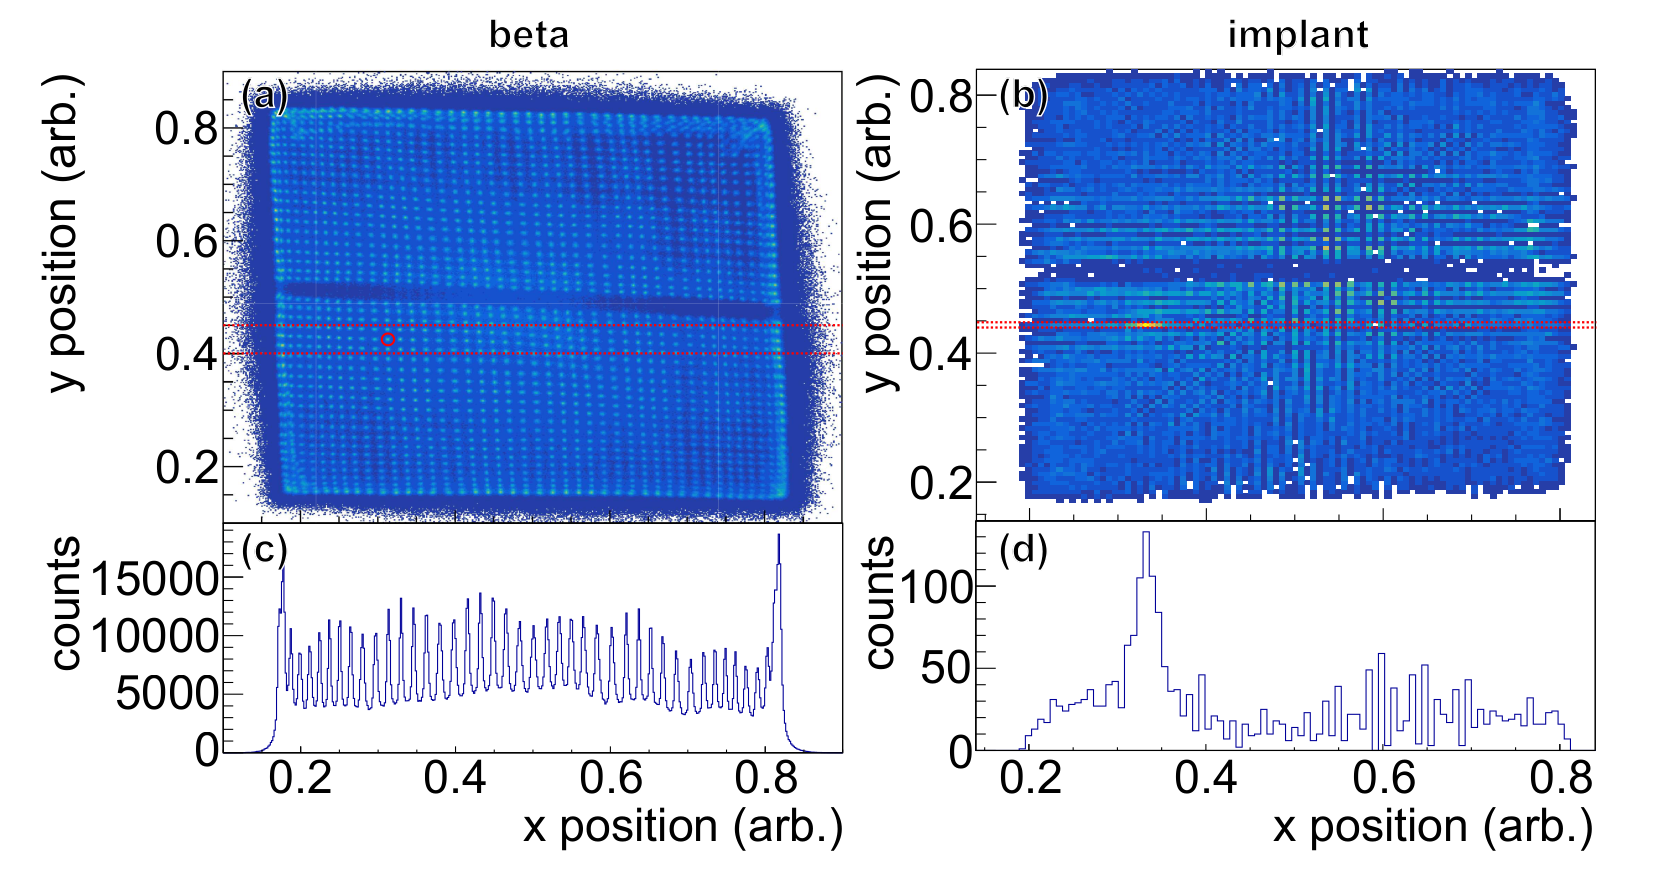
\includegraphics[width=17cm,height=8cm]{figures/ion_beta_correlations.png}
    \caption[YSO x-y images of (a) $\beta$ events and (b) implantation events correlated]{YSO x-y images of (a) $\beta$ events and (b) implantation events correlated to the $\beta$ events in a segment shown in the red circle in panel (a). (c) and (d) are the projection of (a) and (b), respectively, on to the x axis in the cut shown by the red dashed lines \citep{yso2018}.}
\label{fig:ysocorrelations}
\end{figure}

\newpage
\begin{figure}[h!]
    \centering
    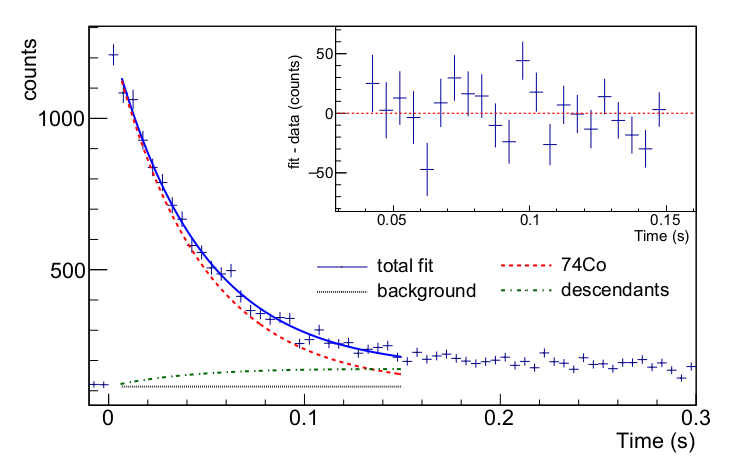
\includegraphics[width=15cm,height=10cm]{figures/half_life.png}
    \caption[The decay curve of the $\beta$ rays from \textsuperscript{74}Co decays]{The decay curve of the $\beta$ rays from \textsuperscript{74}Co decays. The solid blue curve represents the fitting function. The dashed red curve shows the decay component of the parent nucleus,
\textsuperscript{74}Co. The dashed-dotted green curve is the sum of the daughter and neutron-daughter branches. The dotted black line shows the linear background. The plot at the right top of the
figure shows the difference between the data points and the
fitting function \citep{yso2018}.}
    \label{fig:yso_halflife}
\end{figure}

\pagebreak

\section{Delayed Neutron Emission Spectroscopy using \textbf{VANDLE} at RIBF, RIKEN}
Versatile Array of Neutron Detectors at Low Energy (VANDLE) comprises a set of elongated neutron detectors capable of detecting neutrons having the energy of the order of MeV. The individual detector is made up of Eljen-EJ200 organic scintillator bar, coupled to PMT on both sides to collect the light produced. Based on the dimension of the scintillator used, the individual detectors are classified small, medium, and large. VANDLE offers good timing and spatial resolution \citep{VANDLE} for measuring neutrons. For the experiment, a set of 48 medium ($3 \times$ 6 $\times$ 180 $cm^{3}$) arranged in a semi-circular fashion with a diameter 210 cm was implemented. Two high purity germanium clovers and a total of 10 LaBr\textsubscript{3} detectors were placed around YSO to capture decay based $\gamma$-excitations. Signals from all the detectors were read-out using digital electronics modules called Pixie-16 \citep{PIXIE16} by XIA. Each of the modules has 16 channels with four Field Programmable Gate Arrays (FPGA), and a fast built-in Analog to Digital Conversion (ADC) at the rate of 250 Mega samples per second. The experiment took place at RIBF factory at RIKEN Nishina Center, Japan in December 2018. The experiments involved accelerating \textsuperscript{238}U upto 345 MeV/nucleon with a charge state of (86+) which is the primary beam, followed by hitting a 4 mm thick rotating target of \textsuperscript{9}Be, with primay beam intensity peaking $\sim$ 45 pnA. The in-beam fission fragments were selected to be in and around the vicinity of \textsuperscript{78}Ni by the BigRIPS \citep{FUKUDA2013323} facility. The whole experimental campaign lasted for about 5.5 days. The data looks promising, and a great deal of new physics about the structural arrangement and evolution of nuclei in the \textsuperscript{78}Ni region is anticipated from the analysis.

\begin{figure}[h]
    \centering
    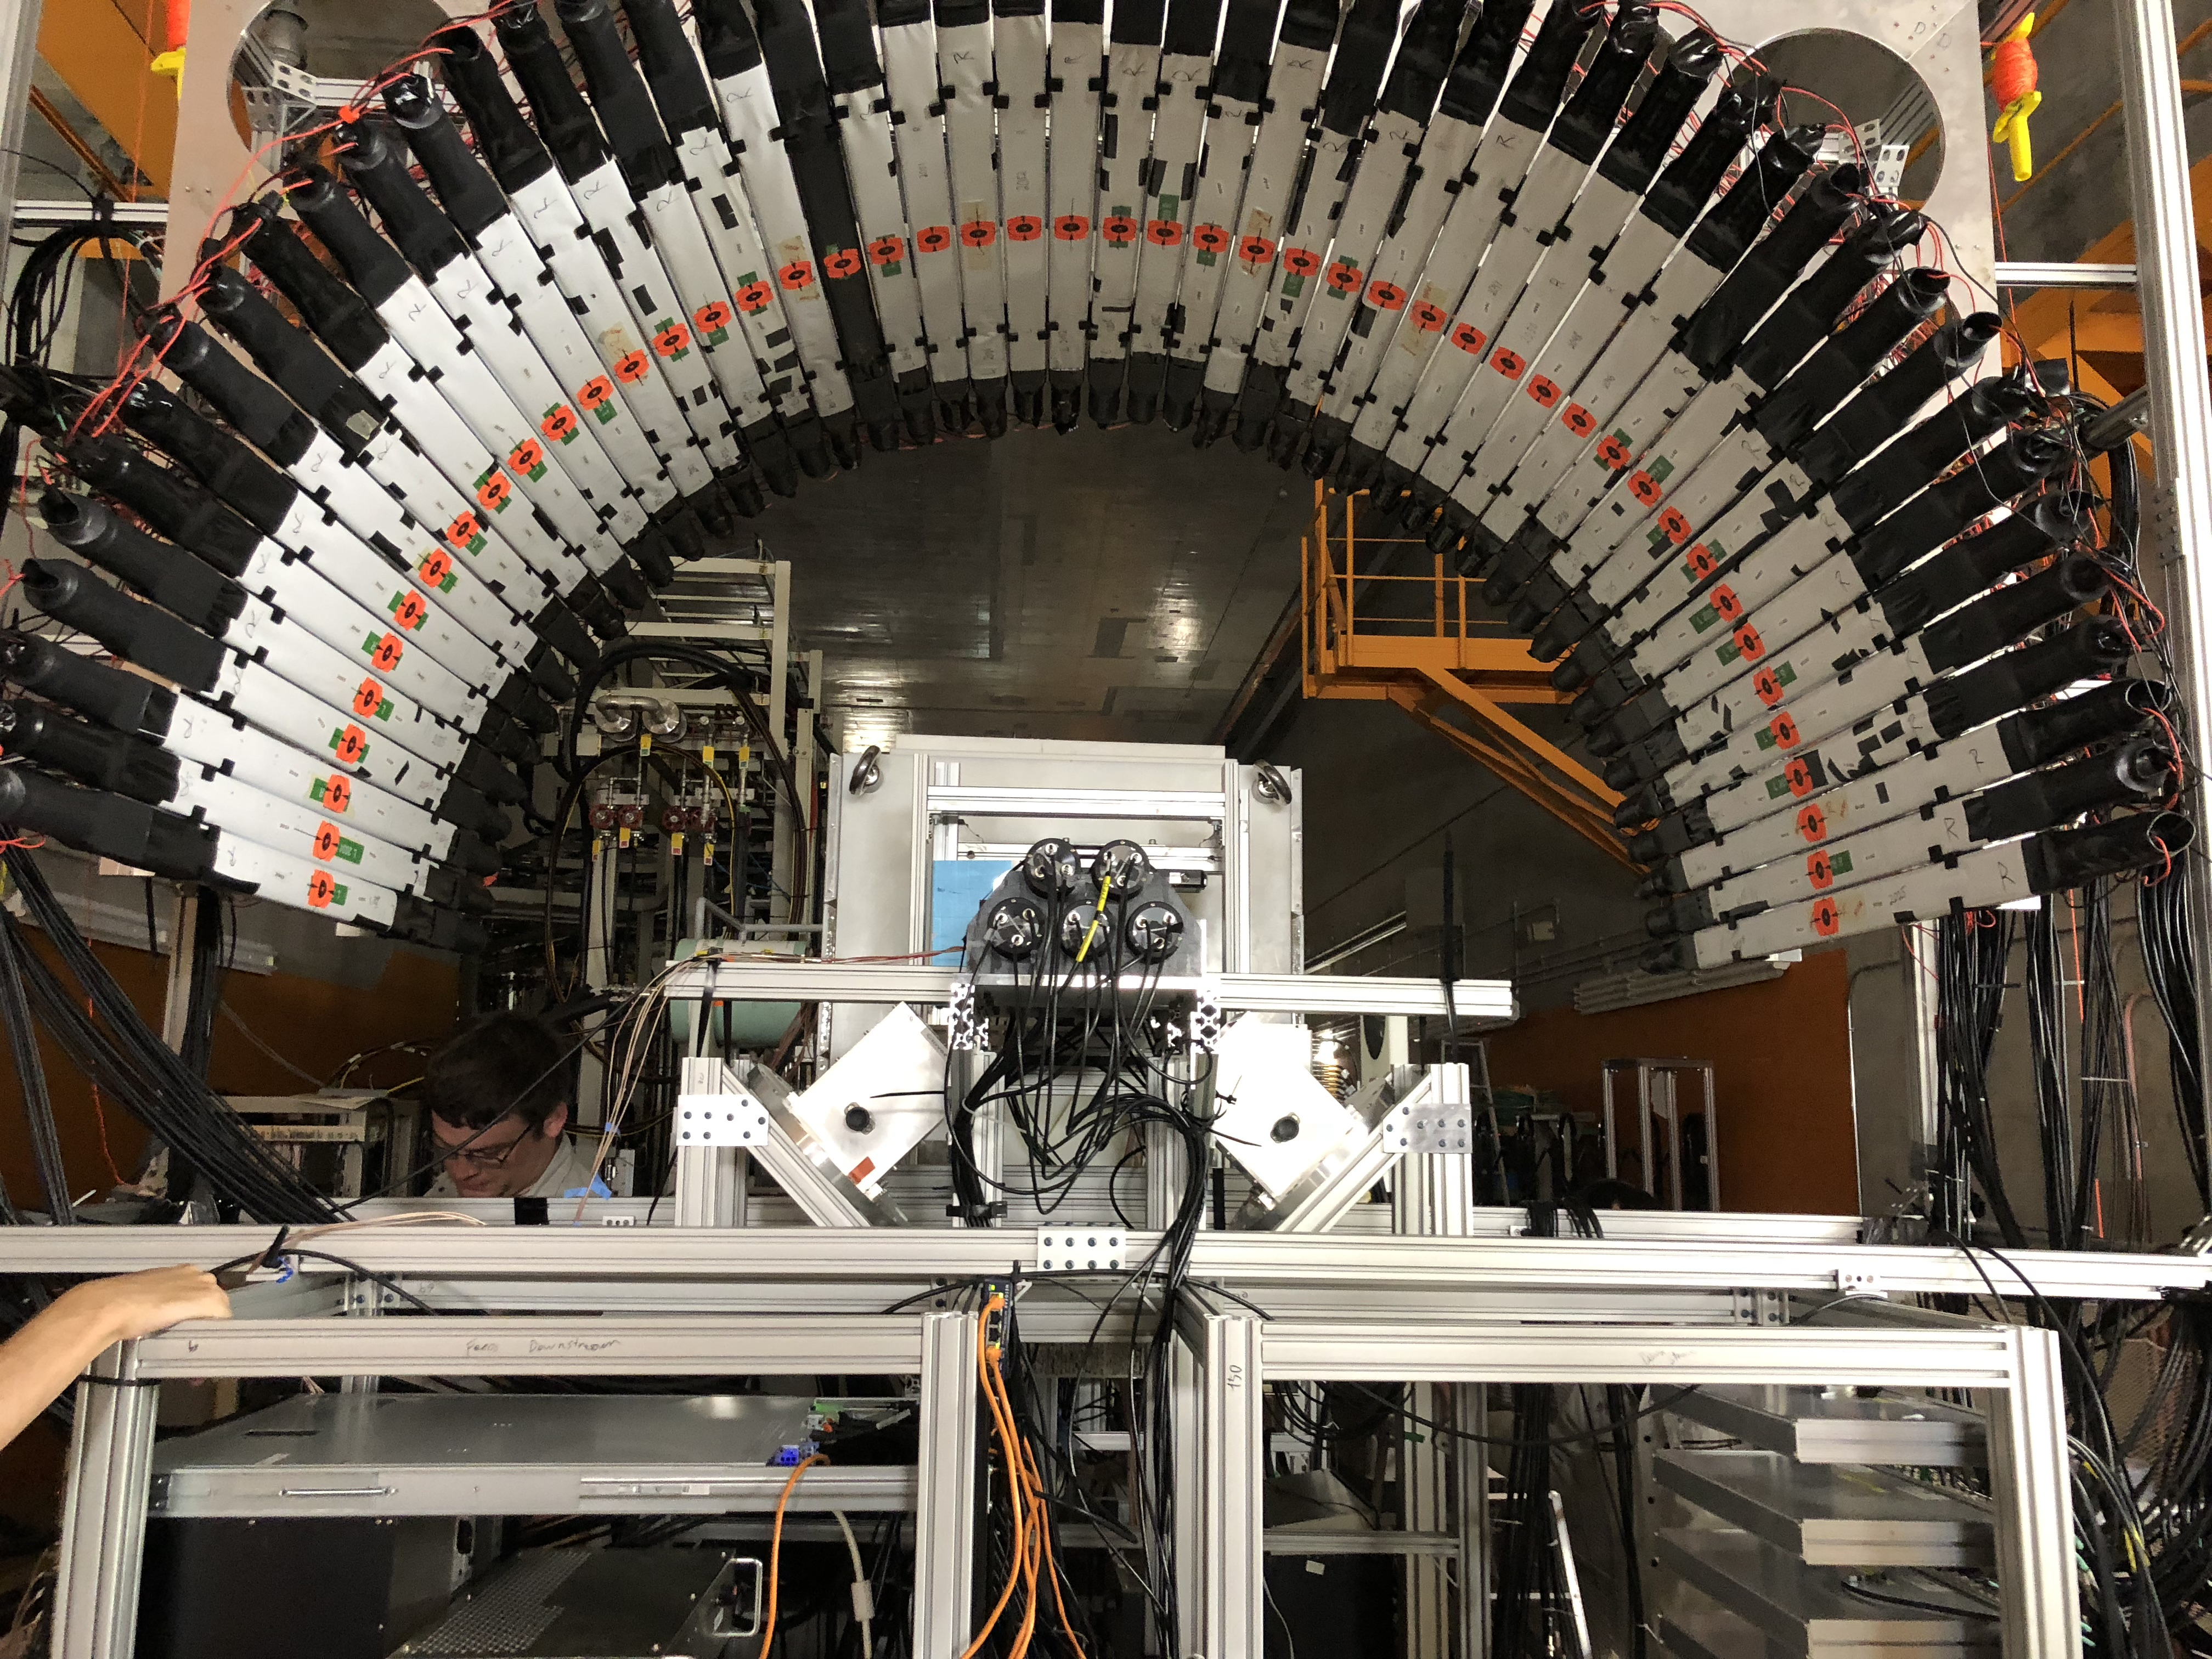
\includegraphics[width=12cm,height=10cm]{figures/vandle_ribf.jpg}
    \caption[The picture shows the site of the experimental setup]{The picture shows the site of the experimental setup at RIBF, RIKEN for the experiment employing VANDLE. The setup was further downstream the F11 focal plane. The setup consists 48 VANDLE bars, YSO (70 $\times$ 70 $\times$ 5  mm\textsuperscript{3}), two high purity germanium clover detectors setup at 90 degrees angle to each other, and 10 LaBr\textsubscript{3} detectors.}
    \label{fig:vandleribf}
\end{figure}


\begin{figure}[h]
	\centering
	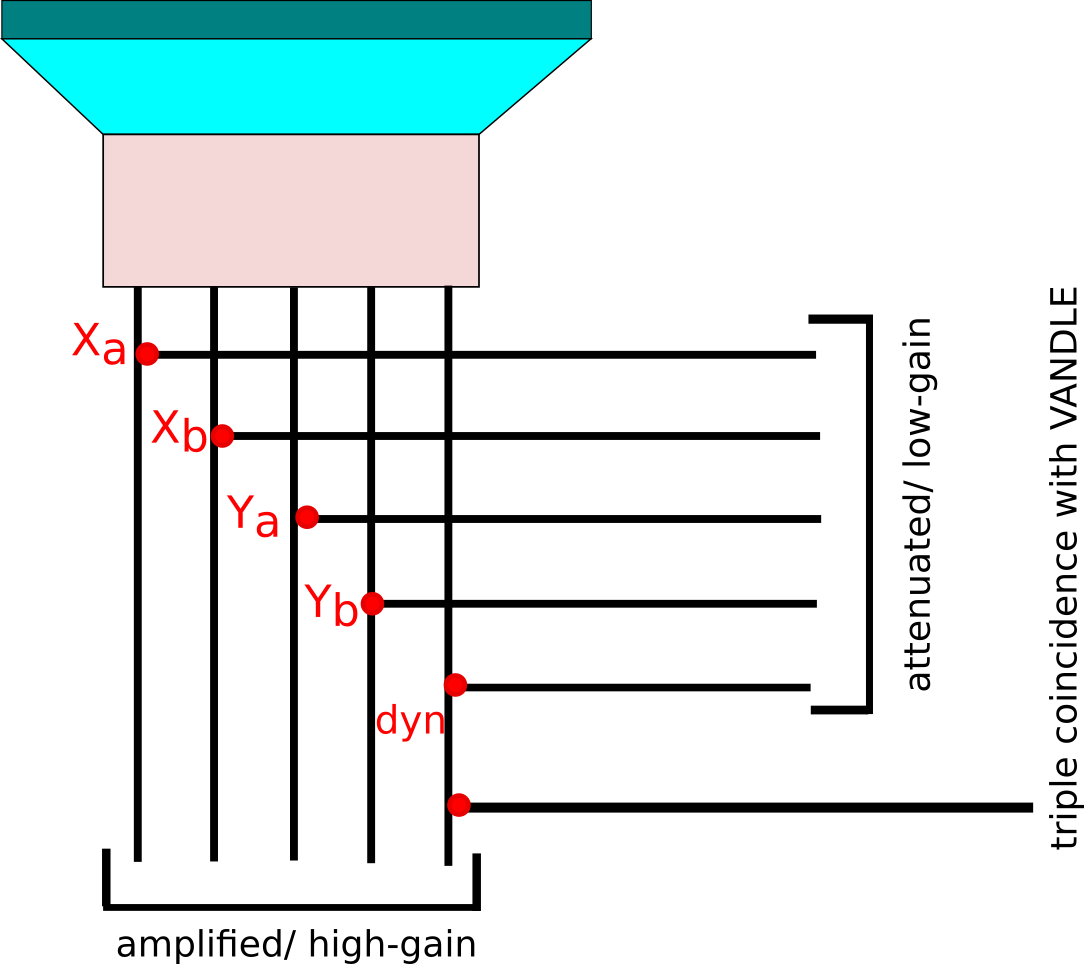
\includegraphics[width=14cm, height=10cm]{figures/YSO_trigger_scheme.png}
	\caption[Division of the 5 YSO signals into low- and high-gain branches]{Division of the 5 YSO signals into low- and high-gain branches. A red dot denote a split in the signal.}
	\label{fig:ysotriggervandle}
\end{figure}

\begin{figure}[h]
    \centering
    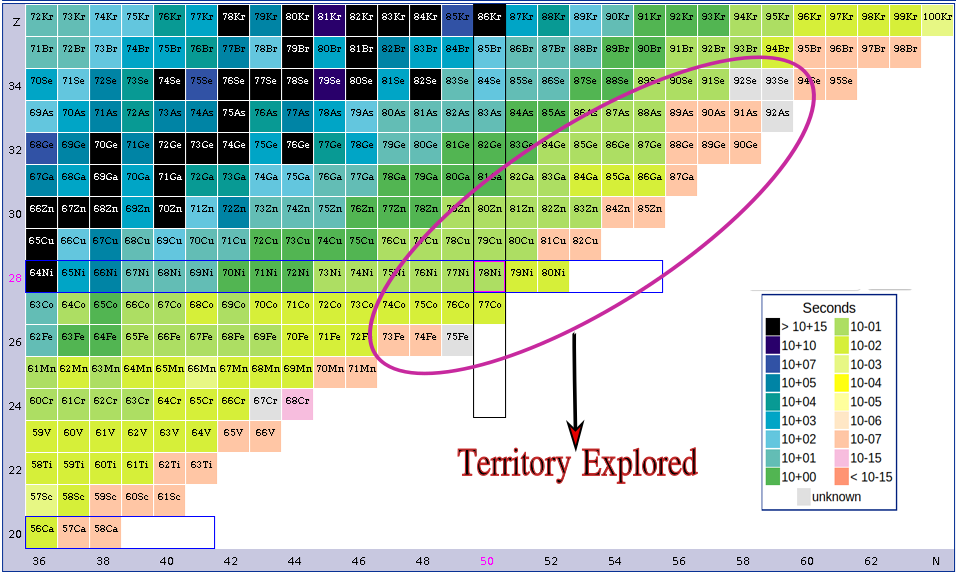
\includegraphics[width=10cm, height=8cm]{figures/nuclie_chart_plot.png}
    \caption[The figure displays a zoomed-in section of nuclei chart]{The figure displays a zoomed in section of nuclei chart, showing the region explored in the experiment, demarcated by a red ellipse.}
    \label{fig:chart_nuclie}
\end{figure}

Provide a block diagram of the setup and explain each component.explain HagRID detectors and what are they made up of. 



\subsection{Trigger Scheme for the experiment}
